\def\year{2021}\relax
%File: formatting-instructions-latex-2021.tex
%release 2021.1
\documentclass[letterpaper]{article} % DO NOT CHANGE THIS
\usepackage{aaai21}  % DO NOT CHANGE THIS
\usepackage{times}  % DO NOT CHANGE THIS
\usepackage{helvet} % DO NOT CHANGE THIS
\usepackage{courier}  % DO NOT CHANGE THIS
\usepackage[hyphens]{url}  % DO NOT CHANGE THIS
\usepackage{graphicx} % DO NOT CHANGE THIS

% ADJUSTED BY AFM ----------------------------------------------------------
\usepackage{amsmath} % ENTERED BY AFM

\urlstyle{rm} % DO NOT CHANGE THIS
\def\UrlFont{\rm}  % DO NOT CHANGE THIS
\usepackage{natbib}  % DO NOT CHANGE THIS AND DO NOT ADD ANY OPTIONS TO IT
\usepackage{caption} % DO NOT CHANGE THIS AND DO NOT ADD ANY OPTIONS TO IT
\frenchspacing  % DO NOT CHANGE THIS
\setlength{\pdfpagewidth}{8.5in}  % DO NOT CHANGE THIS
\setlength{\pdfpageheight}{11in}  % DO NOT CHANGE THIS
\nocopyright
%PDF Info Is REQUIRED.
% For /Author, add all authors within the parentheses, separated by commas. No accents or commands.
% For /Title, add Title in Mixed Case. No accents or commands. Retain the parentheses.
\pdfinfo{
/Title (ML Assignment 1)
/Author (Anthony Menninger)
/TemplateVersion (2021.1)
} %Leave this
% /Title ()
% Put your actual complete title (no codes, scripts, shortcuts, or LaTeX commands) within the parentheses in mixed case
% Leave the space between \Title and the beginning parenthesis alone
% /Author ()
% Put your actual complete list of authors (no codes, scripts, shortcuts, or LaTeX commands) within the parentheses in mixed case.
% Each author should be only by a comma. If the name contains accents, remove them. If there are any LaTeX commands,
% remove them.

% DISALLOWED PACKAGES
% \usepackage{authblk} -- This package is specifically forbidden
% \usepackage{balance} -- This package is specifically forbidden
% \usepackage{color (if used in text)
% \usepackage{CJK} -- This package is specifically forbidden
% \usepackage{float} -- This package is specifically forbidden
% \usepackage{flushend} -- This package is specifically forbidden
% \usepackage{fontenc} -- This package is specifically forbidden
% \usepackage{fullpage} -- This package is specifically forbidden
% \usepackage{geometry} -- This package is specifically forbidden
% \usepackage{grffile} -- This package is specifically forbidden
% \usepackage{hyperref} -- This package is specifically forbidden
% \usepackage{navigator} -- This package is specifically forbidden
% (or any other package that embeds links such as navigator or hyperref)
% \indentfirst} -- This package is specifically forbidden
% \layout} -- This package is specifically forbidden
% \multicol} -- This package is specifically forbidden
% \nameref} -- This package is specifically forbidden
% \usepackage{savetrees} -- This package is specifically forbidden
% \usepackage{setspace} -- This package is specifically forbidden
% \usepackage{stfloats} -- This package is specifically forbidden
% \usepackage{tabu} -- This package is specifically forbidden
% \usepackage{titlesec} -- This package is specifically forbidden
% \usepackage{tocbibind} -- This package is specifically forbidden
% \usepackage{ulem} -- This package is specifically forbidden
% \usepackage{wrapfig} -- This package is specifically forbidden
% DISALLOWED COMMANDS
% \nocopyright -- Your paper will not be published if you use this command
% \addtolength -- This command may not be used
% \balance -- This command may not be used
% \baselinestretch -- Your paper will not be published if you use this command
% \clearpage -- No page breaks of any kind may be used for the final version of your paper
% \columnsep -- This command may not be used
% \newpage -- No page breaks of any kind may be used for the final version of your paper
% \pagebreak -- No page breaks of any kind may be used for the final version of your paperr
% \pagestyle -- This command may not be used
% \tiny -- This is not an acceptable font size.
% \vspace{- -- No negative value may be used in proximity of a caption, figure, table, section, subsection, subsubsection, or reference
% \vskip{- -- No negative value may be used to alter spacing above or below a caption, figure, table, section, subsection, subsubsection, or reference

\setcounter{secnumdepth}{0} %May be changed to 1 or 2 if section numbers are desired.

% The file aaai21.sty is the style file for AAAI Press
% proceedings, working notes, and technical reports.
%

% Title

% Your title must be in mixed case, not sentence case.
% That means all verbs (including short verbs like be, is, using,and go),
% nouns, adverbs, adjectives should be capitalized, including both words in hyphenated terms, while
% articles, conjunctions, and prepositions are lower case unless they
% directly follow a colon or long dash


%Example, Single Author, ->> remove \iffalse,\fi and place them surrounding AAAI title to use it
\title{
Machine Learning - CS 7641
Assignment 2
	
}
\author {
    % Author
    Anthony Menninger \\
}

\affiliations{
    Georgia Tech OMSCS Program \\
    amenninger3\\
    tmenninger@gatech.edu

}

\begin{document}

\maketitle

\begin{abstract}
This paper first reviews three optimization problems using four different algorithms. The algorithms considered are Random Hill Climbing, Simulated Annealing, Genetic Algorithm and MIMIC.  The Four Peaks problem highlights Genetic Algorithm, the K Colors problem highlights MIMIC and the Knapsack Problem highlights Simulated Annealing.  The paper then reviews using Random Hill Climbing, Simulated Annealing, Genetic Algorithm for learning neural network weights for the MNIST image dataset and compares these results to using Back propagation.  
\end{abstract}

\section{Introduction}
The core library used in the experiments in this paper is mlrose [3].  This was developed by Georgia Tech students to support this class by providing a comprehensive tools set for reviewing randomized optimization.  I used the mlrose-hiive [2] fork, which has had other students fix bugs and enhance functionality.  All functions take a seed value which allows random functions to be repeated.  This was used and is documented in the code.

Each problem was reviewed at 3 bit string sizes.   A length of 30 represents a state size of roughly 1 billion, a length of 60 a state size of 10 raised to the 18th, and a length of 90 a state size of 10 raised to the 27th power.  The bit string length of 30 was used to do an original survey of the algorithms and problem.  The 60 bit length was used for tuning and some algorithmic review.  Finally, the bit string length of 90 was used for comparison purposes between the algorithms.  These are very large state spaces which effectively demonstrate the algorithms strengths. 

\section{Four Peaks and the Genetic Algorithm}
\begin{figure}[!htb]
\centering
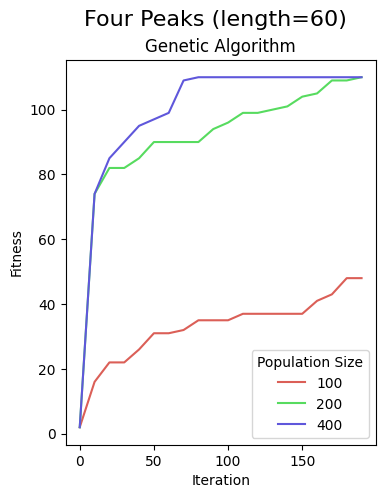
\includegraphics[width=2.75in, height=2.75in]{figures/Four_Peaks_length=60_Genetic_Algorithm_l_60_ma_60_p_100__200__400_mu_0.1_.png}
\caption{Four Peaks Genetic Algorithm:  This shows the fitness curves at different population sizes. Each iteration had a maximum of 60 attempts to find a better solution and a mutation rate of 0.1. }
\label{fig:four_peaks_ga}
\end{figure}

The Four Peaks problem is a simple problem, with fitness growing as consecutive 0's are added to the beginning of a bit string or consecutive 1's to the end.  In addition, there is a bonus if both the leading 0's and trailing 1's exceed a threshold.  This problem creates a very strong locality in the bit string, which will favor the Genetic Algorithms strength.  

The Genetic Algorithm has two key parameters for optimization.  The population size is the number of active states that are considered in each iteration, where each iteration creates a new generation.  The new generation children are  created through combining parts of the bit strings of the previous generation parents with the highest fitness.  The second parameter is a mutation rate, which is a probability whether each bit in the children is randomly changed.  In this algorithm, exploration is created with crossover combinations and mutation and exploitation is governed by selecting only parents with the highest fitness.

\begin{figure}[!htb]
\centering
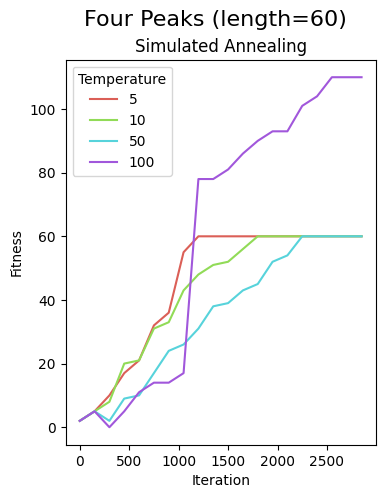
\includegraphics[width=2.75in, height=2.75in]{figures/Four_Peaks_length=60_Simulated_Annealing_l_60_ma_360_d_geom_t_5__10__50__100_.png}
\caption{Four Peaks Simulated Annealing:  This shows the fitness curves at different temperatures using a Geometric Decay schedule. Each iteration had a maximum of 60 attempts to find a better solution. }
\label{fig:four_peaks_sa}
\end{figure}

 \textbf{Figure \ref{fig:four_peaks_ga}} shows the Genetic Algorithm (GA) fitness curve at different population sizes for the Four Peaks problem.  Not surprisingly, the algorithm performs better with larger populations, where there are better chances for breeding successful children.  The algorithm was less sensitive to mutation rates for this problem, with 0.1 performing well, which was then used.



\textbf{Figure \ref{fig:four_peaks_sa}} shows the fitness curve for Simulated Annealing (SA) for different Temperatures.  The temperature governs how likely a candidate instance will be accepted during an iteration if it is not better than the current state instance.  This allows for exploration instead of only finding instances that are better, which is critical to avoid local maxima.    Higher temperatures allow for more exploration, which was necessary for SA to find reach maximum fitness for this problem.  Candidate neighbors are created by looking at local neighbors which only have one bit difference form the current instance.  Another key parameter is how the temperature is decayed in each iteration.  By slowly lowering the temperature, the algorithm is able to settle into the maximum basin instead of getting trapped in a local basin.  Three decay types considered with Geometric decay, Exponential Decay and Arithmetic Decay.  For this problem Geometric performed best at a length of 60 and was used.


\begin{figure}[!htb]
\centering
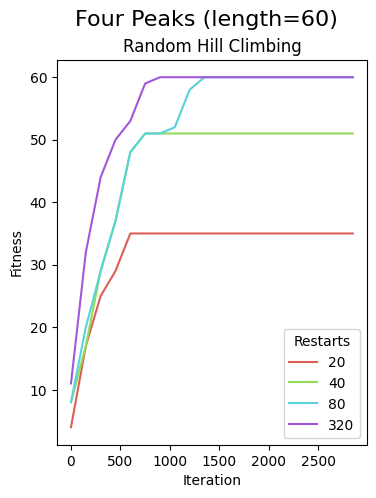
\includegraphics[width=2.75in, height=2.75in]{figures/Four_Peaks_length=60_Random_Hill_Climbing_l_60_ma_120_r_20__40__80__320_.png}
\caption{Four Peaks Random Hill Climbing: Each iteration had a maximum of 60 attempts to find a better solution. }
\label{fig:four_peaks_rhc}
\end{figure}


The Random Hill Climbing (RHC) algorithm looks at local candidate neighbors and at each iteration accepts the first reviewed with better fitness to the current instance.  If there is none better, it assumes this is a maximum.   A key parameter is the number of times the algorithm will restart from different random locations.   Its exploration is limited to the number of random restarts and the number of local neighbors.  It is considered greedy because it only accepts values that are better.

\textbf{Figure \ref{fig:four_peaks_sa}}  shows the results of Random Hill Climbing.  More restarts increases the chance of finding a better solution, but the maximum fitness values are significantly below those of the other algorithms reviewed.

\begin{figure}[!htb]
\centering
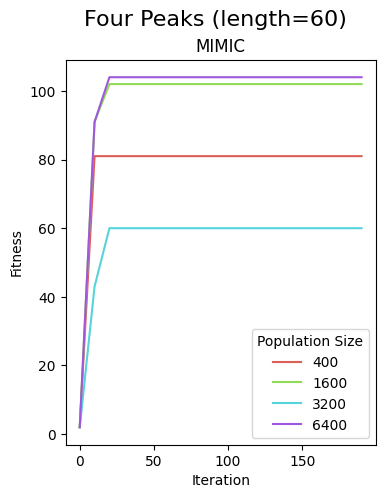
\includegraphics[width=2.75in, height=2.75in]{figures/Four_Peaks_length=60_MIMIC_l_60_ma_60_p_400__1600__3200__6400_k_0.1_.png}
\caption{Four Peaks MIMIC:  This shows the fitness curves at different population size. Each iteration had a maximum of 60 attempts to find a better solution. }
\label{fig:four_peaks_mimic}
\end{figure}

The MIMIC algorithm was created by Professor Isabell Charles.  It uses a population model to create a probability estimation that is refined through each iteration.  The goal is determine underlying structure in the problem through improving the distribution function.

\textbf{Figure \ref{fig:four_peaks_mimic}} shows the MIMIC results.  Like the GA, MIMIC uses a population size, keeping only the fittest in successive iterations.  The figure shows that a population size of 6400 performs best, but that 3200 performs the worst.  Another parameter is the top percentage to keep from one iteration to the next.  A Keep Percentage of 0.3 showed reduced performance, with 0.1 used for the population size reviews. 

\begin{figure}[!htb]
\centering
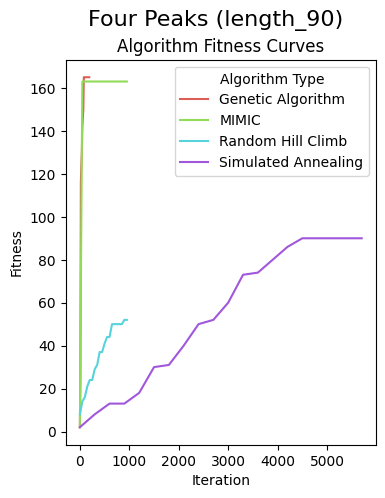
\includegraphics[width=2.75in, height=2.75in]{figures/Four_Peaks_length_90_Algorithm_Fitness_Curves_.png}
\caption{Four Peaks Fitness Comparisons: This shows the fitness curves of the different algorithms using the best tested settings at a bit string length of 90.  }
\label{fig:four_peaks_fitness_comparison_90}
\end{figure}

\begin{figure}[!htb]
\centering
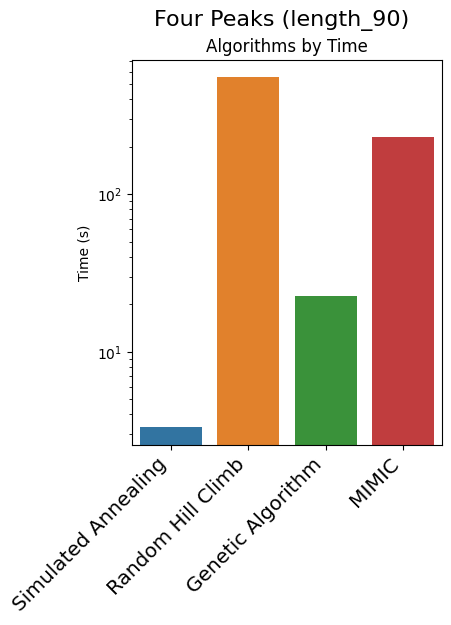
\includegraphics[width=2.75in, height=2.75in]{figures/Four_Peaks_length_90_Algorithms_by_Time_.png}
\caption{Four Peaks Wall Time Comparisons: This shows the time taken to reach the maximum fitness of the different algorithms using the best tested settings at a bit string length of 90.  }
\label{fig:four_peaks_walltime_comparison_90}
\end{figure}

For comparing the algorithms, a bit string length of 90 was used, which is a state space that is a billion times greater than the runs used for the review of individual algorithms.  The Genetic Algorithm provided the maximum fitness, as shown in \textbf{Figure \ref{fig:four_peaks_fitness_comparison_90}}, with only slightly more iterations.  This makes sense given the strong locality of the Four Peaks problem which is the Genetic Algorithms strength.  The MIMIC algorithm is close behind, almost reaching the maximum fitness in a few less iterations than GA.  Simulated Annealing, which is using a hill climbing model with some exploration, is able to find a solution of about half the maximum fitness of GA but taking far more iterations, getting overwhelmed by the enormous state space.  Finally, Random Hill Climbing is not able to reach a comparable fitness level, especially since only 500 restarts were used due to time issues, as seen in next in the review of time.

\textbf{Figure \ref{fig:four_peaks_walltime_comparison_90}} shows another measure of the algorithms, with the wall time to find the best solutions for each algorithm \emph{(Note that the y axis time scale is logarithmic)}. The Genetic Algorithm is almost 20 times faster than MIMIC, even though MIMIC had fewer iterations.  SA was quite fast in spite of the large number of iterations.  Pulling up the rear was Random Hill Climbing, which is slow due to the extended number of iterations it runs with each restart.

\section{Knapsack and Simulated Annealing}
\begin{figure}[!htb]
\centering
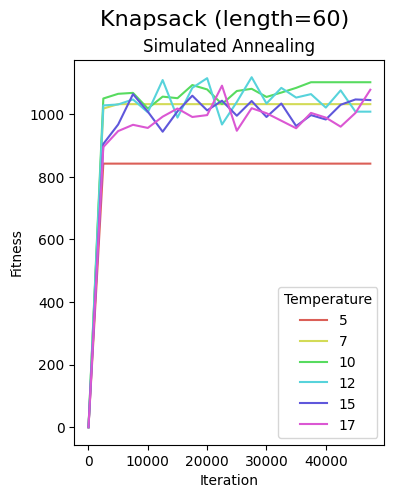
\includegraphics[width=2.75in, height=2.75in]{figures/Knapsack_length=60_Simulated_Annealing_l_60_ma_180_d_arith_t_5__7__10__12__15__17_.png}
\caption{Knapsack Simulated Annealing: This shows the fitness curves at different temperatures using an Arithmetic Decay schedule. Each iteration had a maximum of 180 attempts to find a better solution. }
\label{fig:knapsack_sa}
\end{figure}

\begin{figure}[!htb]
\centering
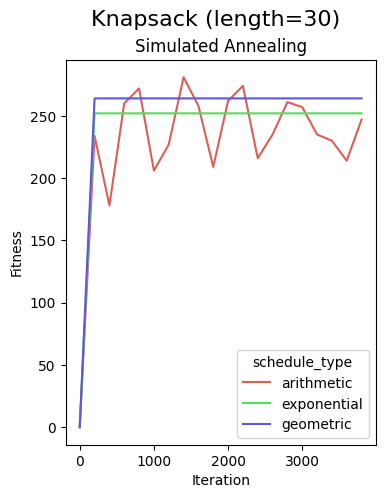
\includegraphics[width=2.75in, height=2.75in]{figures/Knapsack_length=30_Simulated_Annealing_l_30_ma_120_d_geom__arith__exp_t_10_.png}
\caption{Knapsack Simulated Annealing Decay Schedules: This shows the fitness curves using different Decay schedules at a length of 30. Each iteration had a maximum of 120 attempts to find a better solution. }
\label{fig:knapsack_sa_decay}
\end{figure}

\begin{figure}[!htb]
\centering
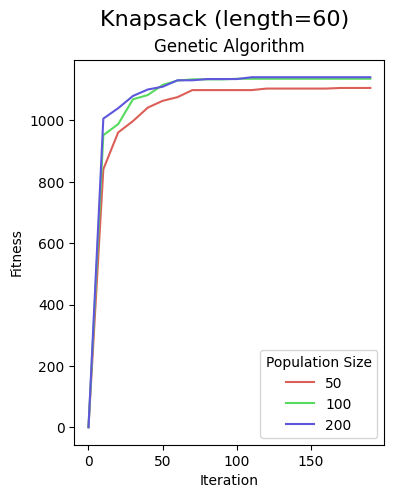
\includegraphics[width=2.75in, height=2.75in]{figures/Knapsack_length=60_Genetic_Algorithm_l_60_ma_60_p_50__100__200_mu_0.1_.png}
\caption{Knapsack Genetic Algorithm: This shows the fitness curves at different population sizes using a mutation rate of 0.1. Each iteration had a maximum of 180 attempts to find a better solution. }
\label{fig:knapsack_ga}
\end{figure}

The Knapsack problem considers a set of items that each have a weight and a value.  The items can be added to the backpack until a threshold is reached, with the fitness score being the sum of the values of the added items.  If the sum of the weights exceeds the threshold, the fitness score drops to zero.  This creates a fitness space with lots of discontinuities near the threshold and many basins of attraction that lead to local maxima instead of the global maxima.   Each item's weight and value was selected in a uniform range between 1 and the total number of items.  The threshold was set to 35\% of the sum of all weights.

The bit strings contain somewhat less locality than the Four Peaks problem, but would expect that many of the high value, low weight items to be easy to identify.  The problem would be significantly harder if items were allowed to be selected multiple times, but was kept as a bit string for comparability to the other problems.

\textbf{Figure \ref{fig:knapsack_sa}} shows the Simulated Annealing algorithm at a length of 60 at different temperatures using an arithmetic decay schedule.  Testing showed that the arithmetic decay schedule allowed higher values to be reached as it performed more exploration.  This is because the arithmetic decay reduces the temperature more slowly, allowing more likelihood of accepting a candidate instance with a lower fitness than the current instance, which allows it to get out of local maxima.  \textbf{Figure \ref{fig:knapsack_sa_decay}} shows the comparisons of decay schedules for the smallest problem size with bit string length of 30.  The variation in the fitness of the arithmetic shows the exploration as it moves around, exceeding the geometric and exponential decays that reduce exploration quickly.


\textbf{Figure \ref{fig:knapsack_ga}} shows the Genetic Algorithm fitness curves at different population sizes.  The Genetic Algorithm performed very strongly on this problem, which is likely due to the binary nature.  Low weight high value items are identified and breed into the next round.  Larger population sizes perform better, as expected.  The algorithm might not perform as well if each item was allowed to be included multiple times because it would become more intwined with other values selected in the state space.

\begin{figure}[!htb]
\centering
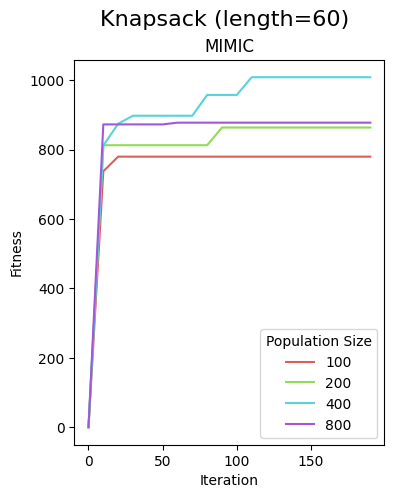
\includegraphics[width=2.75in, height=2.75in]{figures/Knapsack_length=60_MIMIC_l_60_ma_360_p_100__200__400__800_k_0.1_.png}
\caption{Knapsack MIMIC: This shows the fitness curves at different population sizes using a keep percentage of 0.1. Each iteration had a maximum of 360 attempts to find a better solution. }
\label{fig:knapsack_mimic}
\end{figure}

\textbf{Figure \ref{fig:knapsack_mimic}} shows the MIMIC fitness curves at different population sizes.   As in the Four Peaks example, the largest population size was not the best performing.  In addition, the algorithm was not able to reach the same maximum fitness levels that SA and GA did.  This problem has a complicated relationship close to the maximum fitness which was hard for the MIMIC algorithm to optimize fully.  However, it is able to quickly get close to the optimum.

Random Hill Climbing struggled with this problem, as would be expected.  Knapsack has many local maxima as well as many discontinuities, which make it hard to successfully hill climb.   At a bit length of 60, the restart rate would have to be enormous to effectively sample enough of the space to find even modest results.

Further review could be done around the weights, values and thresholds.  In this experiment,  a rather wide range for both weights and values(1 to bit length) was used, with items with large weight and low value clearly not in play.  By narrowing the range, finding the global optimum is likely harder, because more items can participate close to a maximum .

\begin{figure}[!htb]
\centering
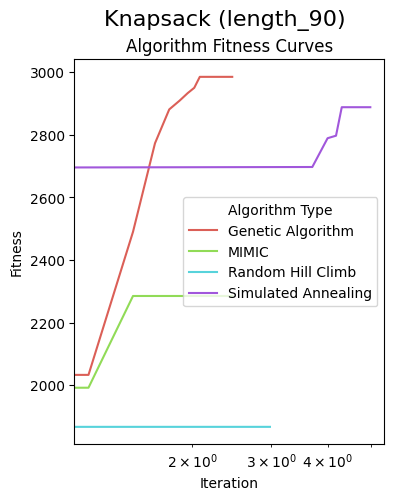
\includegraphics[width=2.75in, height=2.75in]{figures/Knapsack_length_90_Algorithm_Fitness_Curves__log.png}
\caption{Knapsack Fitness Comparisons: This shows the fitness curves of the different algorithms using the best tested settings at a bit string length of 90. \emph{(Note that the x axis iteration scale is logarithmic)} }
\label{fig:knapsack_fitness_comparison_90}
\end{figure}

\begin{figure}[!htb]
\centering
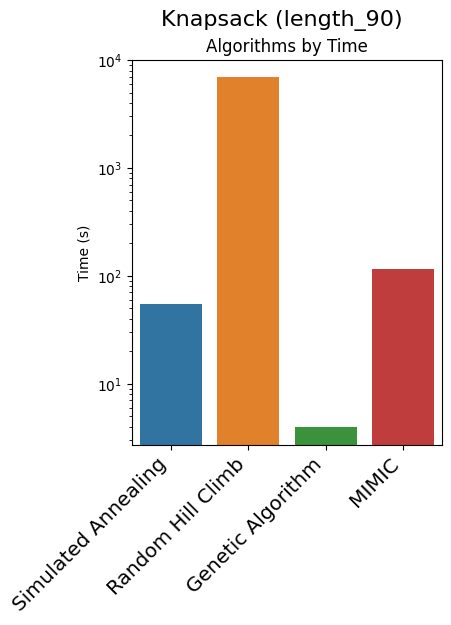
\includegraphics[width=2.75in, height=2.75in]{figures/Knapsack_length_90_Algorithms_by_Time_.png}
\caption{Knapsack Wall Time Comparisons: This shows the time taken to reach the maximum fitness of the different algorithms using the best tested settings at a bit string length of 90.  }
\label{fig:knapsack_walltime_comparison_90}
\end{figure}

\textbf{Figure \ref{fig:knapsack_fitness_comparison_90}} shows the comparison of all the algorithms for the Knapsack problem using a bit string length of 90 \emph{(Note that the x axis iteration scale is logarithmic)} and \textbf{Figure \ref{fig:knapsack_walltime_comparison_90}} shows the wall time comparison for the different algorithms.  Simulated Annealing is able find a good solution, but not the global maximum in a reasonable amount of time. The state space allows SA to explore its way out of local maxima to find better solutions.  GA was the best performing algorithm, reaching the highest fitness in the shortest time.  As discussed earlier, a tighter range on weights and values might make this problem harder for GA.  Finally, Random Hill Climbing was severely challenged in this state space.  

Random Hill Climbing's significant time requirements led to a modest change to the base mlrose-hiive code.  The maximum attempts parameter of the algorithm considered at each iteration to find a better fitness state originally takes a random neighbor for each attempt.  Since the fitness function is deterministic as it the test for RHC, a neighbor needs to be only tested once.  This is in contrast to Simulated Annealing, where a neighbor could be tested multiple times with different results due to the temperature probability of acceptance.  For all bit string cases, the algorithm considers neighbors as strings with one bit changed, so the number of neighbors is the same as the length of the bit string.  Originally, a maximum attempts much larger than the length could be justified in order to reasonably test all the neighbors for RHC.  This added to the time through extra function calls.  My modification randomized the selection of neighbors, but only allowed them to be selected once.  Thus, maximum attempts could be shortened to the length of the bit string.  This was used for RHC in the K Colors problem. 



\section{K Colors and MIMIC}

\begin{figure}[!htb]
\centering
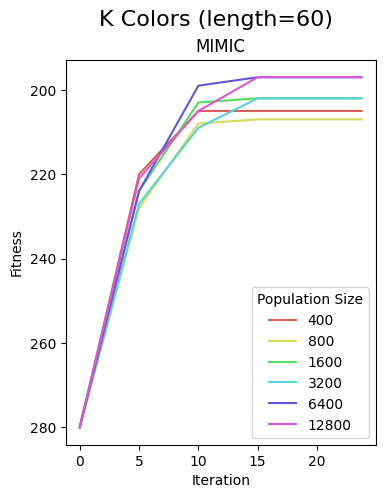
\includegraphics[width=2.75in, height=2.75in]{figures/K_Colors_length=60_MIMIC_l_60_ma_120_p_400__800__1600__3200__6400__12800_k_0.1_.png}
\caption{K Colors MIMIC: This shows the fitness curves at different population sizes using a keep percentage of 0.1. Each iteration had a maximum of 120 attempts to find a better solution. }
\label{fig:kcolor_mimic}
\end{figure}


The K Color problem investigates how a map might be colored so that no contiguous entities use the same color.  It uses a non-directed graph that connects nodes and the fitness function adds one for each edge connecting nodes of the same color.  The goal is to minimize the number of touching colors, so this is a minimization problem instead of a maximization problem.  All algorithms can easily accommodate this by applying a negative to the fitness function.   In using a bit string, we are attempting to arrange two colors to minimize the number of touching similar colors, so we could call this 2 Colors.  My problem generator program creates edges using an edge percentage and each possible edge is then randomly tested.  As in the Knapsack problem, I used a seed for the random generator so that the results are reproducible and comparable between experiments.  I set the edge percentage at 0.35, which provides a complicated topology.  It exhibits some locality, as some edges will connect to nearby bits, but the structure is across the entire bit string.  In addition, the relationship that the structure represents is very straightforward with 2 colors. 

The MIMIC algorithm stands for Mutual-Information-Maximizing Input Clustering.  It randomly samples from the input state space in regions that are more likely to contain the global maxima, using a density estimator function with a given threshold.  MIMIC then uses the randomly generated points to improve the density estimation function and raise the threshold, with this process repeating to raise the threshold and find fitter candidates.  MIMIC is especially well fitted to the K Color problem because  it calculates its probabilities using unconditional probabilities of each feature and pair wise conditional probability between each feature pair.  It is that later that matches almost exactly with the structure of the K-Color problem, where the structure is each edge between two features.  

\textbf{Figure \ref{fig:kcolor_mimic}} shows the fitness curves at different population sizes for MIMIC with a K Color problem of length 60  \emph{(Note that the y axis fitness scale is inverted)}.  It is extremely effective, finding the best solution in less than 15 iterations with a population size as small as 1600.  In the Knapsack problem, the MIMIC algorithm was able to narrow down the key features to focus on, but its unconditional and pairwise conditional probabilities were challenged to make sense of a summation function over all selected features. The K Colors problem maps almost directly into MIMIC's internal model as seen in the low iterations needed to find the optimal solution. 

\begin{figure}[!htb]
\centering
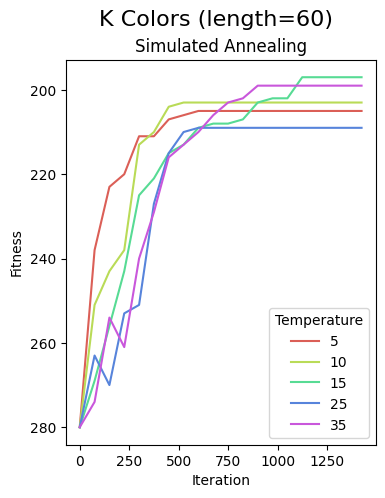
\includegraphics[width=2.75in, height=2.75in]{figures/K_Colors_length=60_Simulated_Annealing_l_60_ma_300_d_geom_t_5__10__15__25__35_.png}
\caption{K Colors Simulated Annealing: This shows the fitness curves at different temperatures with a geometric decay. Each iteration had a maximum of 120 attempts to find a better solution. }
\label{fig:kcolor_sa}
\end{figure}

\textbf{Figure \ref{fig:kcolor_sa}} shows the fitness curve for Simulated Annealing at different temperatures using geometric decay.  The fitness surface for the K Colors problem is relatively smooth and fairly traversable with hill climbing methods.  A high enough temperature allows enough exploration to get out of local maxima, but the smoother surface was most successful using Geometric decay.  Arithmetic decay allowed for too much exploration.


\begin{figure}[!htb]
\centering
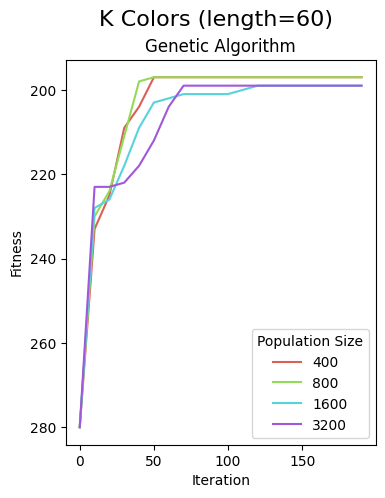
\includegraphics[width=2.75in, height=2.75in]{figures/K_Colors_length=60_Genetic_Algorithm_l_60_ma_120_p_400__800__1600__3200_mu_0.1_.png}
\caption{K Colors Genetic Algorithm: This shows the fitness curves at different population sizes using a mutation rate of 0.1. Each iteration had a maximum of 120 attempts to find a better solution. }
\label{fig:kcolor_ga}
\end{figure}

\textbf{Figure \ref{fig:kcolor_ga}} shows the fitness curve for the Genetic Algorithm at different population sizes using a mutation rate of 0.1.   The GA performs very well on this problem, better than I expected because I thought the locality would be less.  Further review could be done to explore the relationship between GA performance and the number of edges.  

\begin{figure}[!htb]
\centering
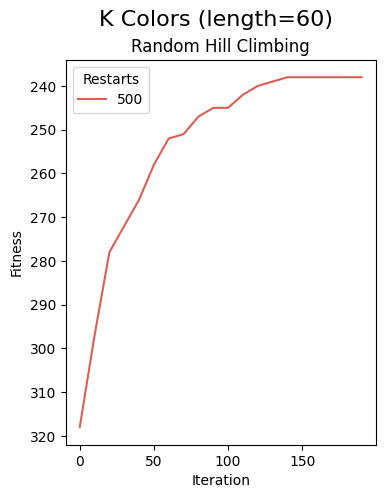
\includegraphics[width=2.75in, height=2.75in]{figures/K_Colors_length=60_Random_Hill_Climbing_l_60_ma_60_r_500_.png}
\caption{K Colors Random Hill Climbing: This shows the fitness curve. Each iteration had a maximum of 60 attempts to find a better solution using the modified mlrose code, testing each neighbor randomly, but only once. }
\label{fig:kcolor_rhc}
\end{figure}

\textbf{Figure \ref{fig:kcolor_rhc}} shows the fitness curve for Random Hill Climbing using the modified mlrose code, testing each neighbor randomly, but only once, per iteration.  RHC is challenged by this problem because the state space can be jumpy due to the multiple connections a feature might have with other features, leading to many local maxima.  


\begin{figure}[!htb]
\centering
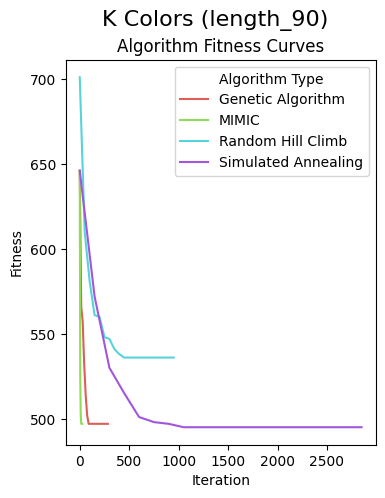
\includegraphics[width=2.75in, height=2.75in]{figures/K_Colors_length_90_Algorithm_Fitness_Curves_.png}
\caption{K Colors Fitness Comparisons: This shows the fitness curves of the different algorithms using the best tested settings at a bit string length of 90. \emph{(Note that the y axis fitness scale, lower is better)} }
\label{fig:kcolor_fitness_comparison_90}
\end{figure}

\begin{figure}[!htb]
\centering
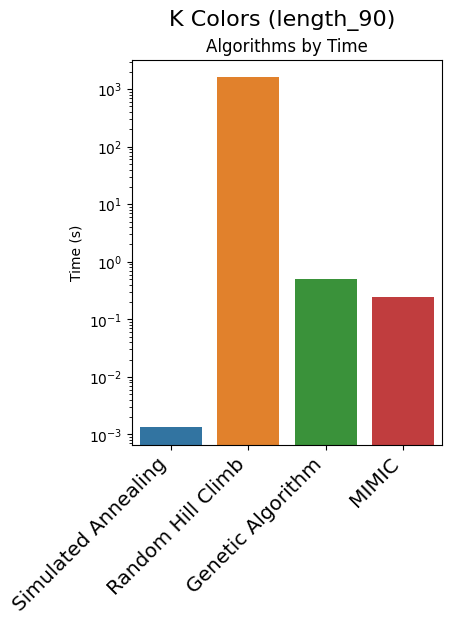
\includegraphics[width=2.75in, height=2.75in]{figures/K_Colors_length_90_Algorithms_by_Time_.png}
\caption{K Colors Wall Time Comparisons: This shows the time taken to reach the maximum fitness of the different algorithms using the best tested settings at a bit string length of 90.  }
\label{fig:kcolor_walltime_comparison_90}
\end{figure}

\textbf{Figure \ref{fig:kcolor_fitness_comparison_90}} shows the comparison of all the algorithms for the K Colors problem using a bit string length of 90 \emph{(Note that the y axis fitness scale, lower is better)} and \textbf{Figure \ref{fig:kcolor_walltime_comparison_90}} shows the wall time comparison for the different algorithms.  MIMIC had the fewest iterations, and was slightly faster than the Genetic Algorithm.  MIMIC's better speed than GA was likely due to its pariticular fit for this problem, having it do fewer iterations.  Simulated Annealing had the most iterations to reach the best fitness, but was the quickest by far, so it would probably be considered the best.  RHC was very challenged by the large state space, taking the longest time and having the worst fitness score.

\section{Neural Network Optimization}

The data set used for the Neural Network Optimization is the MNIST Database of Handwritten Digits [2].  This consists of instances of 28 X 28 greyscale images of the digits 0-9.  One transformation performed was that the values where scaled to 0 to 1, from 0 to 255.  The images were flattened, creating 784 features, one for each pixel.  There are 60,000 training instances and 10,000 test instances.  The dataset is balanced, with roughly equal numbers of examples for each for the digits.  The features can be thought of as related to each other, as they are all positional in a two dimensional grid, with the flattening making this a bit more challenging to interpret, but clearly a high locality in the features.  

I chose to use my PyTorch model from the first assignment with some changes.  I removed one of the hidden layers to make it more manageable to work with the randomized algorithms, with a structure of 784 inputs fully connected to one hidden layer with 84 nodes, fully connected to an output layer with 10 nodes for one hot encoding.  I used a cross entropy loss because of the use of the one hot output labels.


\begin{figure}[!htb]
\centering
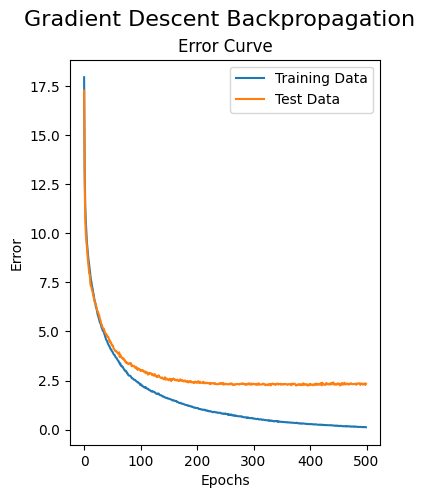
\includegraphics[width=2.75in, height=2.75in]{figures/Gradient_Descent_Backpropagation__epoch_count_500_Error_Curve.png}
\caption{Neural Network Back Propagation Learning Curve: This shows the error rate of the training data and the validation data (test).  The MNIST data is used, flatting the images to 784 features with a network of 84 hidden nodes and 10 one hot outputs for each digit.  }
\label{fig:nn_gradient_initial}
\end{figure}

For training, I used random mini-batches of 100 for each iteration of training.  This created 600 iterations to complete an epoch where the model had done a full pass on the data.  I used a learning rate of 0.001 with the SGD optimizer, which uses stochastic gradient descent with momentum.  This is one of the simpler optimizers and a reasonable comparison to the randomized options. The new network performed well, as seen in  \textbf{Figure \ref{fig:nn_gradient_initial}}  using the standard back propagation, reaching accuracy in the test set of ~97\% within 150 iterations.   The networks from the previous assignment performed better, but had two layers, with even better performance using two convolutional layers. 

Making adjustments to the PyTorch model to allow for the randomized algorithms began with creating functions to get the weights and biases from the networks and then load them after optimization.  The first layer had 65856 weights and 84 biases, the second layer had 840 weights and 10 biases, for a total of 66790 features in the state.  This is quite a large set and I expected the learning algorithms to be challenged by it.  Then I needed to expose a fitness function that would take a proposed state.  To accomplish this, the model takes the proposed state, loads it into the network, and returns the cross entropy loss against the current training batch.   Because this was a loss, the optimization problem is for minimization.

Due to the dramatic impact that different random starting states can have, all experiments loaded the network with the same initial random sets of weights and biases.

I then needed to incorporate the randomized algorithms. I used the mlrose-hiive[2] for the three core algorithms.  All problems would need a problem optimizer, in this case for continuous problems. It was set to minimize the solution, with a minimum possible feature value of -10, a maximum of 10 and a step amount for testing neighbors of 0.1.  The 0.1 functions in some way as a learning rate by limiting how much change can happen at once.  The fitness function used was highlighted earlier.

I needed to replace the Back propagation training for each algorithm using the same mini-batch training. I started with Random Hill Climbing (RHC) where the key settings are maximum iterations, maximum attempts and restarts.  I left restarts at 1 to simplify the activity.  For each iteration, RHC would attempt to change 1 feature, increasing or decreasing it by the step amount.  If the change lowered fitness, it was accepted and RHC moved to the next iteration.  If it did not lower fitness, another attempt was made, up to the maximum attempts.  Thus, each training could only change up to the number of iterations out of a total of 66,790.  With a setting of 20 iterations, with each epoch having 600 trainings, only 12,000 settings could be adjusted each epoch.  This is compared with all weights and biases being updated for each training \emph{iteration} using back propagation.

\begin{figure}[!htb]
\centering
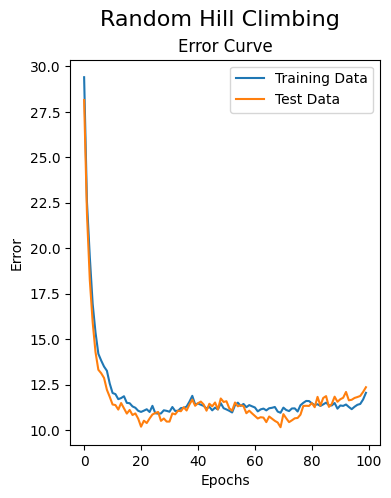
\includegraphics[width=2.75in, height=2.75in]{figures/Random_Hill_Climbing__algorithm_rhc_epochs_100_restart_1_max_iters_20_max_attempts_10_seed_1_capture_iteration_values_False_Error_Curve.png}
\caption{Neural Network Random Hill Climbing Learning Curve: This shows the error rate of the training data and the validation data (test).  Random mini batches of 100 were used, creating 600 iterations per epoch.  Random Hill Climbing used 20 iterations with a maximum attempts per iteration of 10 for each iteration.  }
\label{fig:nn_rhc_initial}
\end{figure}

Using a setting of 20 iterations and 10 maximum attempts, RHC was very effective in the beginning of training, as shown in \textbf{Figure \ref{fig:nn_gradient_initial}}.  The time per epoch increased by about a factor of 20, which was expected given the significant extra gyrations performed.  My biggest surprise was how well it performed!  While it only gets to an accuracy of about 88-89\%, it does this in about 25-30 epochs, which seems quite quick.  I think the fitness space for neural network is pretty smooth, which means that RHC stands a good chance to climb effectively.  Looking more closely, RHC is changing only about 7 features per iteration, much less than the potential 20, in the beginning of training.  This slowly drops as the training continues and it becomes more difficult to find upward progress.  

Also, I initially attempted to use a seed for the random state of the RHC algorithm to allow for reproducibility.  However, using the same seed caused it to choose the same features each time, preventing learning.  I adjusted this to use the seed to set a random generator for the mlrose algorithm.

Another consideration is how complicated the model is.   The sum of the absolute values of all the weights of the RHC network is 11,448.  The back propagation sum was 2,245.  The back propagation model is changing almost all the weights at each iteration, but is doing so in a proportional manner that should continue to lessen change.  The RHC makes almost the same change at each iteration, with the only shrinking being the fact it makes fewer changes as training goes along.  Overall, the model with small weights is preferred and will likely generalize better. 

There are several areas that might enhance the RHC model. First, lowering the step might improve performance, similar to lowering the learning rate of back propagation.  More interesting would be to lower the step amount as training progresses,  much as learning rates are often decayed over training.  Another idea would be to increase the maximum attempts as training goes on.  Finding a state with better fitness becomes more difficult as training goes along. With such a large number of features,  this would possibly allow for a better solution.  Finally, tuning of the mini batch setting may also be helpful.  With back propagation, results may often improve with lower learning rates at the expense of more training iterations.  Learning can be slowed by having bigger batches, causing fewer updates per epoch.  

Fundamentally, the challenge that RHC will have is getting stuck in is local minima.  It does not have a structured way to get out of these.  A large step size in a sense might help, by stepping out of local minima, but those same large steps make it unlikely it can perform fine tuned optimization and require it to go to ever larger weights.   


\begin{figure}[!htb]
\centering
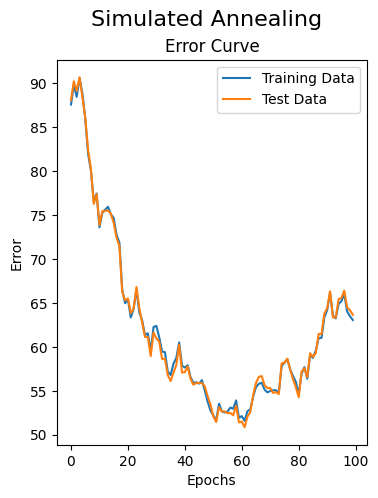
\includegraphics[width=2.75in, height=2.75in]{figures/Simulated_Annealing__algorithm_sa_epochs_100_temperature_0.01_decay_geom_max_iters_20_max_attempts_5_seed_1_.png}
\caption{Simulated Annealing Learning Curve: This shows the error rate of the training data and the validation data (test).  Random mini batches of 100 were used, creating 600 iterations per epoch.  Simulated Annealing started with a temperature of 0.01, used geometric decay,  20 iterations with a maximum attempts of 10 for each iteration.  }
\label{fig:nn_sa_initial}
\end{figure}

Simulated Annealing at first glance seems to offer some solution to the challenge of local minima found in RHC and initially I expected it to perform better.  Quickly, it became clear that it performed worse as seen in \textbf{Figure \ref{fig:nn_sa_initial}}.  Temperature was set to the lowest setting of 0.001, but learning was slower than RHC and ultimately undid itself after about 60 iterations.  The key challenge comes from the fact that even with a low temperature, the SA accepts all iterations, with an average of 20 changes for 20 iterations.  It is exploring too much and not exploiting enough, with a total sum of weights at the end of 100 epochs of 22,445, about twice as much as RHC. 

\begin{figure}[!htb]
\centering
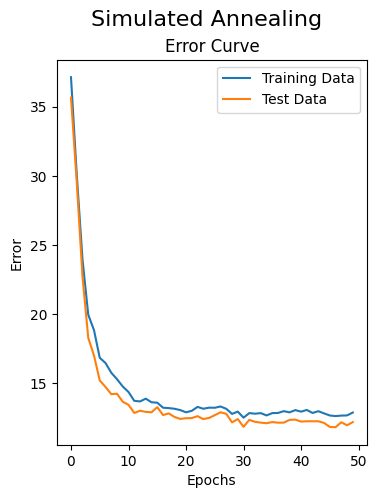
\includegraphics[width=2.75in, height=2.75in]{figures/Simulated_Annealing__epochs_50_temperature_0_0001_min_temp_1e_06_decay_geom_max_iters_20_max_attempts_5_seed_1_Error_Curve.png}
\caption{Simulated Annealing Learning Curve with Lower Temperature:  The same settings were used as in the previous figure except that the initial temperature was much lower at 0.0001.  }
\label{fig:nn_sa_adjusted}
\end{figure}

I added the ability to lower the minimum temperature and another run was done for 50 epochs, using a much lower starting temperature of 0.0001, as seen in  \textbf{Figure \ref{fig:nn_sa_adjusted}}.  This performed much better, but had a weights sum of 14331after just 50 epochs.  It seems like it was still exploring too much, accepting an average of 16 changes our of 20. 

Simulated Annealing's challenge in this setting is that it uses the same starting temperature for each epoch run.  Temperature decay means initial training mini batches have easier acceptance and higher exploration while later mini batches have lower exploration.  Exploration would ideally would be lower in the initial training epochs to make progress quickly,  higher in the middle epochs to explore the space a bit, then lower again to move towards the best solution, instead of becoming more restrictive inside each epoch, then resetting.

\begin{figure}[!htb]
\centering
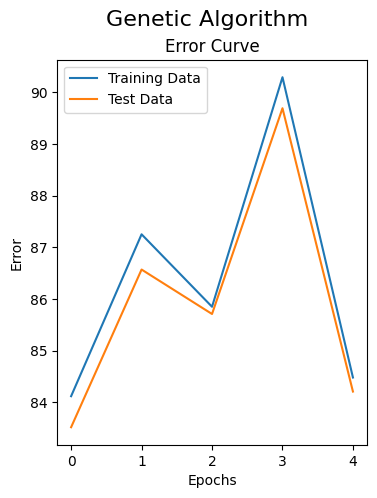
\includegraphics[width=2.75in, height=2.75in]{figures/Genetic_Algorithm__algorithm_ga_epochs_5_max_iters_3_max_attempts_3_seed_1_.png}
\caption{Genetic Algorithm Learning Curve:  A population size of 100 with a mutation rate of 0.01 was used.  Only 5 iterations were done due to the significant time used by the algorithm.  }
\label{fig:nn_ga}
\end{figure}

Genetic Algorithms was a big star in the initial optimization problems, but was likely going to be challenged with the neural network.  Earlier, using only bit strings meant that cross over was more likely to be successful because the optimal value for each feature was going to be a 1 or a 0.  With a continuous state, optimal values could be anything, which means randomly switching sections of the state was less likely to be effective.  In addition, the key nature of locality comes to the fore here.  It does not make any sense that we would switch the weights of the last layer with a some sub section of the first layer and expect improvement, especially considering that they impact each other. 

 \textbf{Figure \ref{fig:nn_ga}} shows GA's challenge.   With error between 84\% and 90\%, it performing barely above chance where we would expect error of 90\%.  Due to crossover, every feature is changing at each iteration step.   The sum of the weights reaches 331,874 after 5 epochs, showing unsupportable growth.  This algorithm takes 70 times longer than RHC or SA, which themselves were 20 times longer than back propagation.
 
I don't have many ideas to improve GA's performance because its fundamental model doesn't make much sense for network weights.  Possibly removing mini batches and training the entire data set in each iteration might help a bit, but I am skeptical.


Table with best score, times, weights

Did use Pytorch, run.  Switched over to mlrose


\section{References}
\begin{tabular}{l p{2.75in}}
\\
1 & The MNIST Database of Handwritten Digits. url: http://yann.lecun.com/exdb/mnist/.
\\
2 & Rollings, A. (2020). mlrose: Machine Learning, Randomized Optimization and SEarch package for Python, hiive extended remix. https://github.com/hiive/mlrose. Accessed: 2/11/2022
\\
3 & Hayes, G. (2019). mlrose: Machine Learning, Randomized Optimization and SEarch package for Python. https://github.com/gkhayes/mlrose. Accessed: 2/11/2022.
\\
4 & Menninger, A. (2022)  Code created for this experiment https://github.com/gkhayes/mlrose. Accessed: 2/11/2022.
\end{tabular}
\end{document}
